\chapter {Element Attributes}
\label{c:attrib}
\index{Element attribute}

%-----------------------------------------------------------------
\section{Dependent and Independent Attributes} 
\label{s:depend} 
\index{Element attribute!dependent and independent}

\index{Parameter statement}
For convenience, \bmad computes the values of some attributes based
upon the values of other attributes. These dependent variables are
listed in Table~\ref{t:dependent}. Also shown in
Table~\ref{t:dependent} are the independent variables they are
calculated from.  In the table \vn{n_part} and \vn{l_lattice} (lattice
length) are lattice attributes, not element attributes. The first two
are set by the \vn{parameter} statement (See
\sref{s:param}). \vn{l_lattice} is calculated when the
lattice is read in.

\index{BBI_const}\index{Charge}\index{Sig_x}\index{Sig_y}
\index{Beam_energy}\index{N_part}\index{E_field}\index{Voltage}
\index{Hkick}\index{Vkick}\index{Gap}\index{L}
\index{Beam_energy}\index{E_loss}\index{Delta_e}\index{Gradient}
\index{L}\index{Rho}\index{Angle}\index{L_chord}
\index{G}\index{L}\index{K1}\index{Rho}
\index{B_max}\index{Beam_energy}\index{BeamBeam}\index{Elseparator}
\index{Lcavity}\index{Rbend}\index{Sbend}\index{Wiggler}
\begin{table}[h]
\centering {
\begin{tabular}{|l|l|l|} \hline
{\em Element}                 & {\em Dependent Variables}    & {\em Independent Variables}  \HH
 \vn{BeamBeam}                & \vn{bbi_const}               & \vn{charge}, \vn{sig_x}, \vn{sig_y}, \vn{beam_energy}, \vn{n_part} \HH
 \vn{Elseparator}             & \vn{e_field}, \vn{voltage}   & \vn{hkick}, \vn{vkick}, \vn{gap}, \vn{l}, \vn{beam_energy}    \HH
 \vn{Lcavity}                 & \vn{e_loss}, \vn{delta_e}    & \vn{gradient}, \vn{l}                           \HH
 \vn{Rbend}, \vn{Sbend} & \vn{rho}, \vn{angle}, \vn{l_chord} & \vn{g}, \vn{l}                                  \HH
 \vn{Wiggler} (periodic type) & \vn{k1}, \vn{rho}            & \vn{b_max}, \vn{beam_energy}                    \HH
\end{tabular}
}
\caption[Table of dependent variables.]{Table of dependent variables and 
  the independent variables 
they are calculated from.}
\label{t:dependent}
\end{table}

\index{Lattice!expansion}\index{Harmon}\index{Delta_e}\index{Gradient}
\index{Rho}\index{G}\index{Angle}\index{Rf_frequency}
No attempt should be made to set or vary within a program dependent
attributes. It should be remarked that this is not an iron clad rule.
If a program properly bypasses \bmad's attribute bookkeeping routine
then anything is possible. Before lattice expansion \bmad allows the
setting of a select group of dependent variables if the appropriate
independent is left unspecified.  The list of settable dependent
variables is given in Table~\ref{t:dep_except}.  After reading in the
lattice \bmad will set the appropriate independent variable based
upon the value of the dependent variable. \vn{harmon} is the exception in 
that it will never be set by the bookkeeping routine.
\index{Lcavity}\index{Rbend}
\index{Sbend}\index{RFcavity}
\begin{table}[h]
\centering {
\begin{tabular}{|l|l|l|} \hline
{\em Element}            & {\em Dependent Variable Set}  &  {\em Independent Variables Not Set} \HH
  \vn{Lcavity}           & \vn{delta_e}       & \vn{gradient}  \HH
  \vn{Rbend}, \vn{Sbend} & \vn{rho}           & \vn{g}         \HH
  \vn{Rbend}, \vn{Sbend} & \vn{angle}         & \vn{g}         \HH
  \vn{RFcavity}          & \vn{rf_frequency}  & \vn{harmon}    \HH
\end{tabular}
}
\caption {Dependent variables that can be set in a primary lattice file.}
\label{t:dep_except}
\end{table}

\index{G}\index{B_field}
\index{B_gradient}\index{Ks}
\index{K1}\index{K2}\index{K3}
\index{BL_kick}\index{BL_hkick}\index{BL_vkick}
\index{Kick}\index{HKick}\index{VKick}
The normal attribute used to vary the strength of, say, a
\vn{quadrupole} is \vn{k1}.  It is sometimes convenient to be able to
vary the magnetic field strength directly instead. To do this \bmad
has a rule that if the appropriate field attribute appears in the
primary lattice file then it becomes an independent variable and the
normalized strength attribute (the strength attribute normalized by
the reference energy) becomes a dependent variable as tabulated in
Table~\ref{t:dep_field}.
\index{Sbend}\index{Rbend}\index{Solenoid}\index{Quadrupole}
\index{Sol_Quad}\index{Sextupole}\index{Octupole}
\begin{table}[h]
\centering {
\begin{tabular}{|l|l|l|} \hline
  {\em Element} & {\em Normalized Strength Attribute} & {\em Field Attribute} \HH
  \vn{Sbend}, \vn{Rbend}     & \vn{g}      &  \vn{b_field}       \HH
  \vn{Solenoid}              & \vn{ks}     &  \vn{b_field}       \HH
  \vn{Sol_quad}              & \vn{ks}     &  \vn{b_field}       \HH
  \vn{Sol_quad}              & \vn{k1}     &  \vn{b_gradient}    \HH
  \vn{Quadrupole}            & \vn{k1}     &  \vn{b_gradient}    \HH
  \vn{Sextupole}             & \vn{k2}     &  \vn{b_gradient}    \HH
  \vn{Octupole}              & \vn{k3}     &  \vn{b_gradient}    \HH
  \vn{HKicker}, \vn{VKicker} & \vn{kick}   &  \vn{bl_kick}       \HH
  Most                       & \vn{hkick}  &  \vn{bl_hkick}      \HH
  Most                       & \vn{vkick}  &  \vn{bl_vkick}      \HH
\end{tabular}
}
\caption {Field and Strength Attributes.}
\label{t:dep_field}
\end{table}
Using both field strength and normalized strength as the independent
variable for a given element is not permitted. For example, for a quadrupole the 
normalized strengths \vn{k1}, \vn{hkick}, and \vn{vkick} can be used as the
independent variable or the field strengths \vn{b_gradient}, \vn{bl_hkick} and
\vn{bl_vkick}. but the mixing of the two is not valid
\begin{example}
  Q1: quadrupole, k1 = 0.6, bl_hkick = 37.5  ! NO. Not VALID.
\end{example}
To define an element with the field strength as the independent
attribute without setting the strength just set the strength to zero. For example
\begin{example}
  Q1: quadrupole, b_gradient = 0   ! Field strengths now the independent variables
\end{example}


%-----------------------------------------------------------------
\section{Type, Alias and Descrip Attributes}
\label{s:string}
\index{Type|textbf}
\index{Alias|textbf}
\index{Descrip|textbf}

There are three string labels associated with any element:
\begin{example}
  type    = <String>
  alias   = <String>
  descrip = <String>
\end{example}
\bmad routines do not use these labels except when printing element
information. \vn{type} and \vn{alias} can be up to 16 characters in
length and \vn{descrip} can be up to 200 characters. The attribute
strings can be enclosed in double quotation marks ("). The attribute
strings may contain blanks. If the attribute string does not contain a
blank then the quotation marks may be omitted. In this case the first
comma (,) or the end of the line marks the end of the string. Example:
\begin{example}
  Q00W: Quad, type = "My Type", alias = Who_knows, &
                                  descrip = "Only the shadow knows"
\end{example}

%-----------------------------------------------------------------
\section{Beam\_Energy and P0C Attributes}
\label{s:energy}
\index{Parameter statement}\index{Beam_energy}
\index{Energy_start}\index{P0c_start}
\index{Patch}\index{Lcavity}\index{P0c}
The attributes that define the reference energy and momentum at an element are:
\begin{example}
  beam_energy = <Real>  ! Total energy in eV.
  p0c         = <Real>  ! Momentum in eV.
\end{example}
The energy and momentum are defined at the exit end of the element.
For ultra--relativistic particles these two values are the same.
See~\sref{s:phase_space_coords}. These attributes are dependent and thus
cannot be set for an element directly in the lattice input
file. The value of \vn{beam_energy} and \vn{p0c} for an element is calculated by
\bmad to be the same as the previous element except for \vn{Lcavity}
and \vn{Patch} elements. To set the \vn{beam_energy} or \vn{p0c} at the start of
the lattice use the \vn{beginning} or \vn{parameter} statements.
See~\sref{s:param}. Since the energy changes from the start to the end
of an \vn{Lcavity}, An \vn{Lcavity} has the attributes
\begin{example}
  energy_start
  p0c_start
\end{example}
which is just the reference energy and momentum at the start of the element.


%-----------------------------------------------------------------
\section{Offset, Pitch, Tilt, and Roll Attributes}
\label{s:offset}
\index{X_offset|textbf}
\index{Y_offset|textbf}
\index{S_offset|textbf}
\index{X_pitch|textbf}
\index{Y_pitch|textbf}
\index{Roll|textbf}
\index{Tilt|textbf}

There are up to 7 attributes that can offset a physical element
from the reference orbit. They are
\begin{example}
  x_offset = <Real>
  y_offset = <Real>
  s_offset = <Real>
  x_pitch  = <Real>
  y_pitch  = <Real>
  tilt     = <Real>
  roll     = <Real>
\end{example}
\index{Pitch}
The exception here is the \vn{Pitch} element which uses these
attributes to modify the reference orbit itself.

\vn{x_offset} translates an element in the local $x$--direction
as shown in Figure~\ref{f:pitch}. Similarly, \vn{y_offset} and 
\vn{s_offset} translate an element along the local $y$ and 
$z$--directions respectively. For a bend it is assumed that
the bend angle is small and the rotation of the local reference
axes through the bend is ignored.

The \vn{x_pitch} attribute rotates an element about the $y$--axis so
that the exit face of the element is displaced in the $+x$--direction
as shown in figure~\ref{f:pitch}. Similarly the \vn{y_pitch} attribute
rotates an element about the $x$--axis so that the exit face of the
element is displaced in the $+y$--direction. The rotations are about
the center of the element which is in contrast to the \vn{dtheta} and
\vn{dphi} misalignments of \mad which rotate around the entrance
point. In terms of rotation angle
\index{MAD!element rotation origin}
\begin{example}
  x_pitch =  dtheta
  y_pitch = -dphi
\end{example}
In both \bmad and \mad offsets are applied before pitches.
\begin{figure}[ht]
  \centering
  \includegraphics{pitch.eps}
  \caption{Geometry of Pitch and Offset attributes}
  \label{f:pitch}
\end{figure}

\begin{figure}[ht]
  \centering
  \includegraphics{tilt.eps}
  \caption{Geometry of a Tilt}
  \label{f:tilt}
\end{figure}

The tilt attribute rotates the element in the $(x, y)$ plane as
shown in figure~\ref{f:tilt}. For a bend the rotation axis is the
$z$-axis at the entrance face. The reference orbit is also rotated
with the element. A bend with a tilt of $\pi/2$ will bend a beam
upward vertically. The \vn{hkick} and \vn{vkick} attributes are
not affected by \vn{tilt} except for \vn{Kicker} and \vn{ElSeparator}
elements
Like MAD, \bmad allows the use of the \vn{tilt} attribute without
a value to designate a skew element. For example
\begin{example}
  q1: quad, l = 0.6, x_offset = 0.03, y_pitch = 0.001, tilt
\end{example}
Default tilts can be used for \vn{rbend}, \vn{sbend}, \vn{sol_quad},
\vn{quadrupole}, \vn{sextupole}, and \vn{octupole} elements.
The default tilt is $\pi/n$ where $n$ is the number of poles of the
element (bends have 2, quadrupoles have 4, etc.) 


The \vn{roll} attribute is only used for bends
and rotates the bend, along an axis that runs through the entrance
point and exit point as shown in figure~\ref{f:roll}. A \vn{roll} 
does not affect the reference orbit. The major effect of a \vn{roll}
is to give a vertical kick to the beam.
\begin{figure}[ht]
  \centering
  \includegraphics{roll.eps}
  \caption{Geometry of a Roll}
  \label{f:roll}
\end{figure}


%-----------------------------------------------------------------
\section{Hkick, Vkick, and Kick Attributes}
\label{s:kick}
\index{Hkick|textbf}\index{BL_hkick|textbf}
\index{Vkick|textbf}\index{BL_vkick|textbf}
\index{Kick|textbf}\index{BL_kick|textbf}


\index{Hkicker}
\index{Vkicker}
\index{Elseparator}
\index{Kicker}
The kick attributes that an element may have are:
\begin{example}
  kick,  bl_kick  = <Real>  ! Used only with a Hkicker or Vkicker
  hkick, bl_hkick = <Real>
  vkick, bl_vkick = <Real>
\end{example}
\vn{kick}, \vn{hkick}, and \vn{vkick} attributes are the integrated
kick of an element in radians. \vn{kick} is only used for \vn{Hkicker}
and \vn{Vkicker} elements. All other elements that can kick use
\vn{hkick} and \vn{vkick}. The \vn{tilt} attribute will only rotate a
kick for \vn{Hkicker}, \vn{Vkicker}, \vn{Elseparator} and \vn{Kicker}
elements. This rule was implemented so that, for example, the
\vn{hkick} attribute for a skew quadrupole would represent a
horizontal steering. The \vn{bl_kick}, \vn{bl_hkick}, and
\vn{bl_vkick} attributes are the integrated field kick in
\vn{meters-Tesla}. Normally these are dependent attributes except if
they appear in the lattice file (\sref{s:depend}).

%-----------------------------------------------------------------
\section{Aperture and Limit Attributes}
\label{s:limit}
\index{Aperture|textbf}
\index{Limit|textbf}
\index{Aperture_at|textbf}

\begin{figure}[ht]
  \centering
  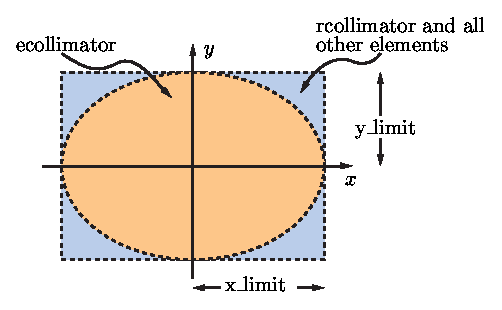
\includegraphics{apertures.eps}
  \caption{Apertures for ecollimator and rcollimator elements}
  \label{f:limit}
\end{figure}

\index{Ecollimator}
\index{Rcollimator}
\index{X_limit}
\index{Y_limit}
\index{X_offset}
The aperture attributes are:
\begin{example}
  x_limit  = <Real>      ! Horizontal limit
  y_limit  = <Real>      ! Vertical limit
  aperture = <Real>      ! Alternative to specifying x_limit and y_limit
  aperture_at = <Switch> ! What end aperture is at.
\end{example}
\vn{x_limit}, \vn{y_limit} specify the half--width of the aperture of
an element as shown in figure~\ref{f:limit}. Notice that an \vn{Ecollimator}
has a elliptical aperture while a \vn{Rcollimator} and all other elements
have rectangular apertures. A zero \vn{x_limit} or
\vn{y_limit} is interpreted as no aperture in the $x$ or $y$
direction. \vn{x_offset} and \vn{y_offset} move the aperture but not
pitches or tilts.

An \vn{aperture} attribute supersedes
any \vn{x_limit} and \vn{y_limit} values and sets \vn{x_limit} and
\vn{y_limit} equal to the value of \vn{aperture}.

\index{Entrance_end}
\index{Exit_end}
\index{Aperture_at}
By default the aperture is evaluated at the exit face only of the
element. This can be changed by setting the \vn{aperture_at} attribute.
Possible settings for \vn{aperture_at} are:
\begin{example}
  entrance_end
  exit_end  ! default
  both_ends
\end{example}
Note that the entrance and exit ends of an element are independent of
which direction particles are tracked through an element. Thus if a
particle is tracked backwards it enters an element at the ``exit end''
and exits at the ``entrance end''.

Example:
\begin{example}
  q1: quad, l = 0.6
  q1[x_limit] = 0.03
  q1[y_limit] = 0.03
  q1[aperture] = 0.03  ! equivalent to the proceeding 2 lines.  
  q1[aperture_at] = both_ends
\end{example}

%-----------------------------------------------------------------
\section{Length Attributes}
\label{s:l}

\index{L}
\index{L_chord}
\index{Rbend}
\index{Sbend}
The length attributes are
\begin{example}
  l       = <Real>  ! 
  l_chord           ! Chord length of a bend. Dependent attribute.
\end{example}
The length \vn{l} is the path length of the reference
particle. The one exception that that for an \vn{Rbend} the length
\vn{l} is the chord length (\sref{s:bend}). Internally, \bmad converts
all \vn{Rbend}s to \vn{Sbend}s and stores the chord length
under the \vn{l_chord} attribute.

\index{Wiggler}
Note that for \vn{Wiggler}s
the length \vn{l} is not the same as the path length for a particle
with the reference energy starting on the reference orbit.

%-----------------------------------------------------------------
\section{Symplectify Attribute}
\label{s:symp}
\index{Symplectify}

The \vn{symplectify} attribute
\begin{example}
  symplectify = <Logical>
\end{example}
is used to make the transfer matrix for an element symplectic. The
linear transport matrix may be non--symplectic for a number of
reasons.  For example, the linear matrix that comes from expanding a
Taylor Map around any point that is not the origin of the map is
generally not symplectic. The transfer matrix for an element can be
symplectified by setting the \vn{symplectify} attribute to True. See
section \ref{s:symp_method} for details on how a matrix is
symplectified. The default value of \vn{symplectify}, if it is not
present, is \vn{False}. If it is present without a value then it
defaults to true. Examples:
\begin{example}
  s1: sextupole, l = 0.34                       ! symplectify = False
  s1: sextupole, symplectify = True, l = 0.34   ! symplectify = True
  s1: sextupole, symplectify, l = 0.34          ! symplectify = True
\end{example}

%-----------------------------------------------------------------
\section{Is\_on Attribute}
\label{s:is_on}
\index{Is_on}

The \vn{is_on} attribute
\begin{example}
  is_on = <Logical>
\end{example}
is used to turn an element off. Turning
an element off essentially converts it into a drift.
Example
\begin{example}
  q1: quad, l = 0.6, k1 = 0.95
  q1[is_on] = False
\end{example}
Note: \vn{is_on} does not affect any apertures that are set.

%-----------------------------------------------------------------
\section{Multipole Attributes: An, Bn, KnL, Tn}
\label{s:multip}

\index{Multipole!an, bn} 
\index{Multipole!KnL, Tn} 
\index{AB_Multipole}
\index{Multipole}
\index{Radius}
A \vn{Multipole} element specifies its multipole components using an
Amplitude (\vn{KnL}) and a tilt (\vn{Tn})
\begin{example}
  KnL = <Real>
  Tn  = <Real>
\end{example}
\vn{AB_Multipole} and all other elements that
have multipole attributes specify the multipoles using normal
(\vn{Bn}) and skew (\vn{An}) components 
\begin{example}
  An = <Real>
  Bn = <Real>
\end{example}
Here \vn{n} ranges from 0
(dipole component) through 20. Example:
\begin{example}
  q1: quadrupole, b0 = 0.12, a20 = 1e7
\end{example}

Multipole formulas for are given in \sref{s:fields}.  Note that for
\vn{Multipole} and \vn{AB_multipole} (but not any other element) a
non-zero dipole component will affect the reference orbit (just like a
normal dipole will).

For everything other than a \vn{Multipole} and \vn{AB_multipole}, the
mutipole strength is scalled by a factor $F \, r_0^{n_\text{ref}} /
r_0^n$ (cf.~\Eq{ababf}) where $F$ is the strength of the element (for
example $F$ is $K1 \cdot L$ for a quadrupole), and $r_0$ is the
``measurement radius'' and is set by the \vn{radius} attribute. The
default value of $r_0$, if the \vn{radius} is not given, is 1.0.
